
\section{Evaluation}

Our experiments are performed on a machine with Intel(R) Xeon (R) CPU E565 2.4GHz in Ubuntu 16.04. 


There are two things to evaluate, the first is the storage overhead, and the second is the time consumed for recovery. It should be noted that storage overhead for logical back up is not the same as the storage overhead in the DBMS since they use different data representation. For example, 64 bits integer should occupy 64 bits in the DBMS, However, in logical backup, integer is stored as string, which means the storage overhead is related to the length of the string. For example, the integer 123456789 can occupy 72 bits. In our evaluation, we compute the storage overhead based on the string representation as the logical backup tool mysqldump do. For time consumpation, we choose to first evaluate each kind of encryption algorithms and then give the estimated time overhead for recovery. We do not evaluate the total time consumpation for recovery since different logical backup tools can have different recovery speed, this speed is influenced by implementation optimizations like multi-threading or batch insert, which are not related to our topic. So we only estimate the time for recovering to the logical representation of the data. 


First, we analyze the overhead of time.  Recall that we may want to remove salt, so we first need to know how fast can we regenerate a new salt. We do experiment with the function in CryptDB and find that the computation overhead for one salt value is around 0.7 $\mu$s. So this computation is quite fast and the overhead could be ignored. We also need to know how much time is consumed to do computation in each layer, so we do experiment for those algorithms.


\begin{figure*}   
  \begin{minipage}[t]{0.5\columnwidth}  
    \centering
    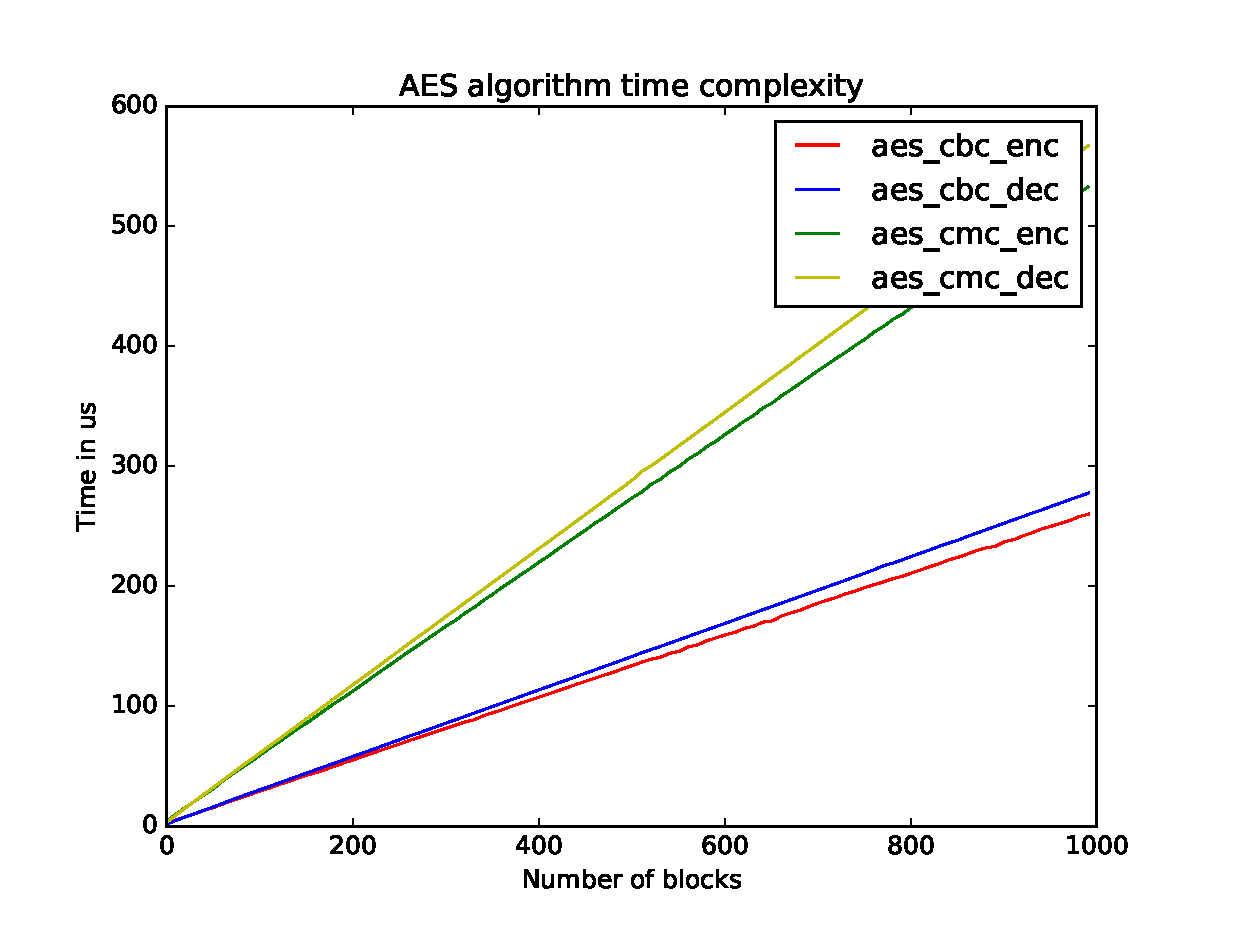
\includegraphics[width=4.7cm]{images/aes.eps}  
     
    \caption{\small{This figure show how the encryption and decryption time change with the input length.}}  
    \label{fig:stack9}   
  \end{minipage}% 
  \hfill  
  \begin{minipage}[t]{0.5\columnwidth}
    \centering   
    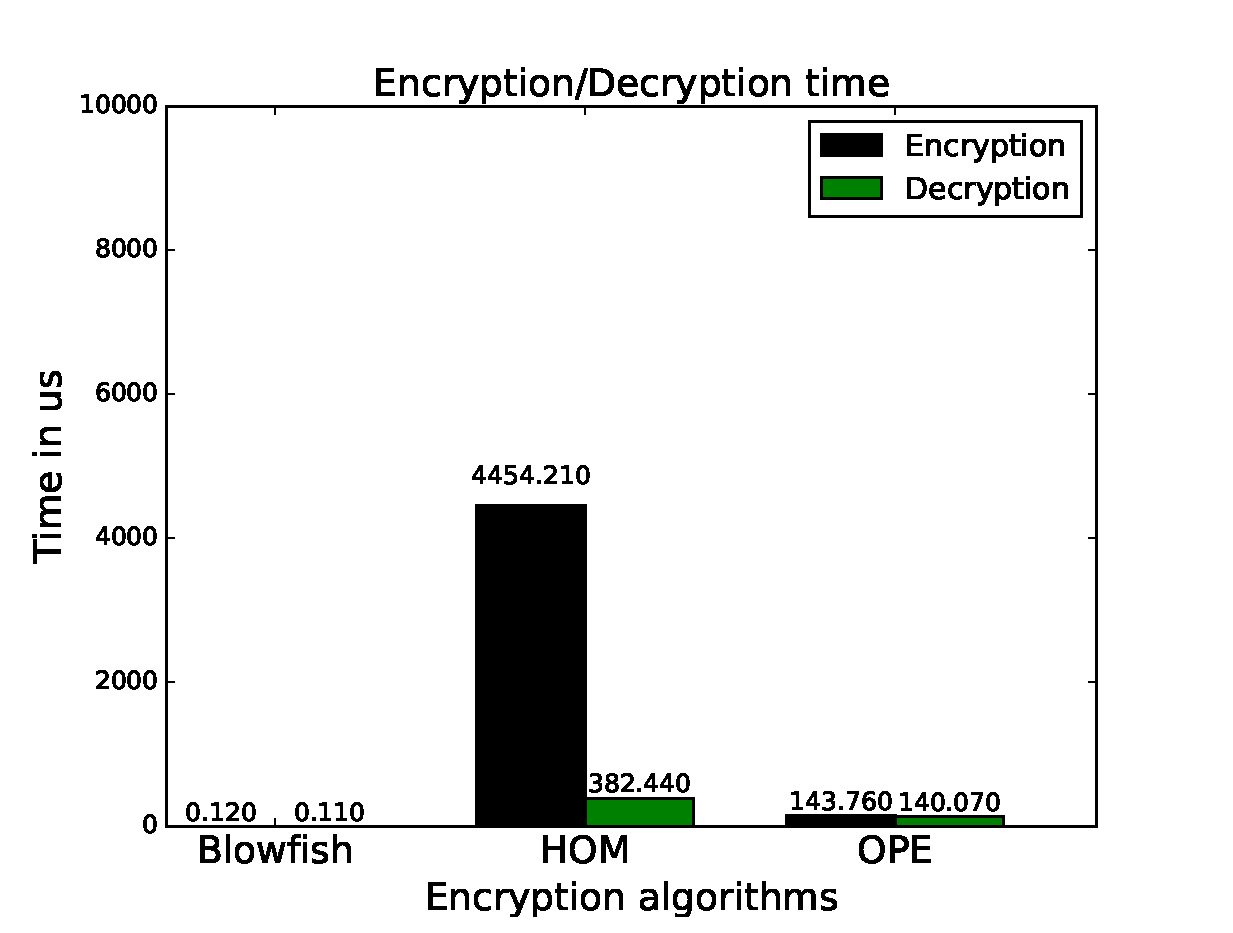
\includegraphics[width=4.7cm]{images/time.eps}   
    \caption{\small{This figures show the encryption and decryption time of the algorithm blowfish, Pailliar, and order preserving encryption}}  
    \label{fig:stack10}   
  \end{minipage}
  \hfill
  \begin{minipage}[t]{0.5\columnwidth}  
    \centering   

    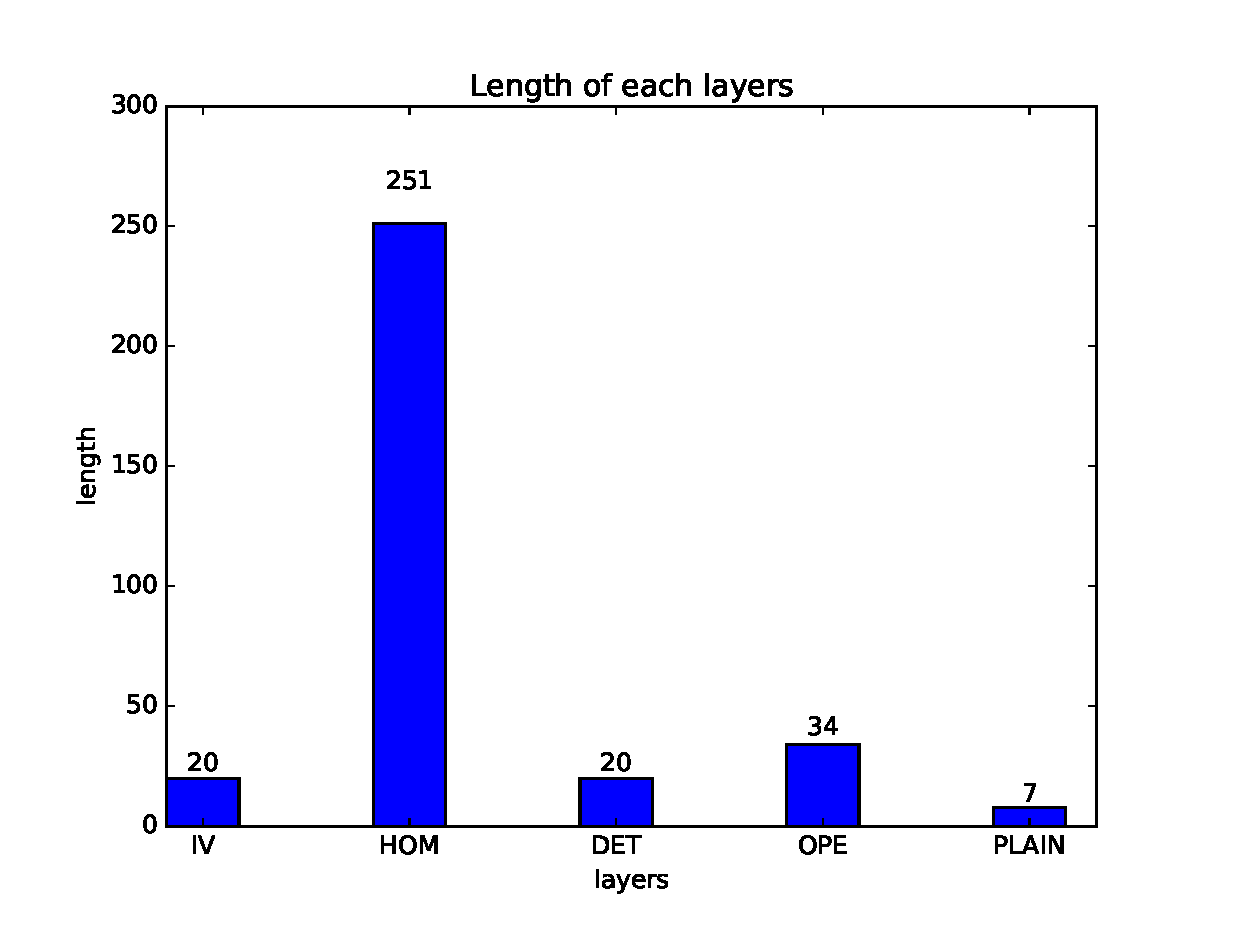
\includegraphics[width=4.7cm]{images/size-of-each-onion.eps}   
    \caption{\small{This figure shows the size of each encrypted column in the form of text file for the table we creates that has one plaintext column of Integer type}} 
    \label{fig:stack11}   
  \end{minipage}%
  \hfill 
  \begin{minipage}[t]{0.5\columnwidth}   
    \centering   
    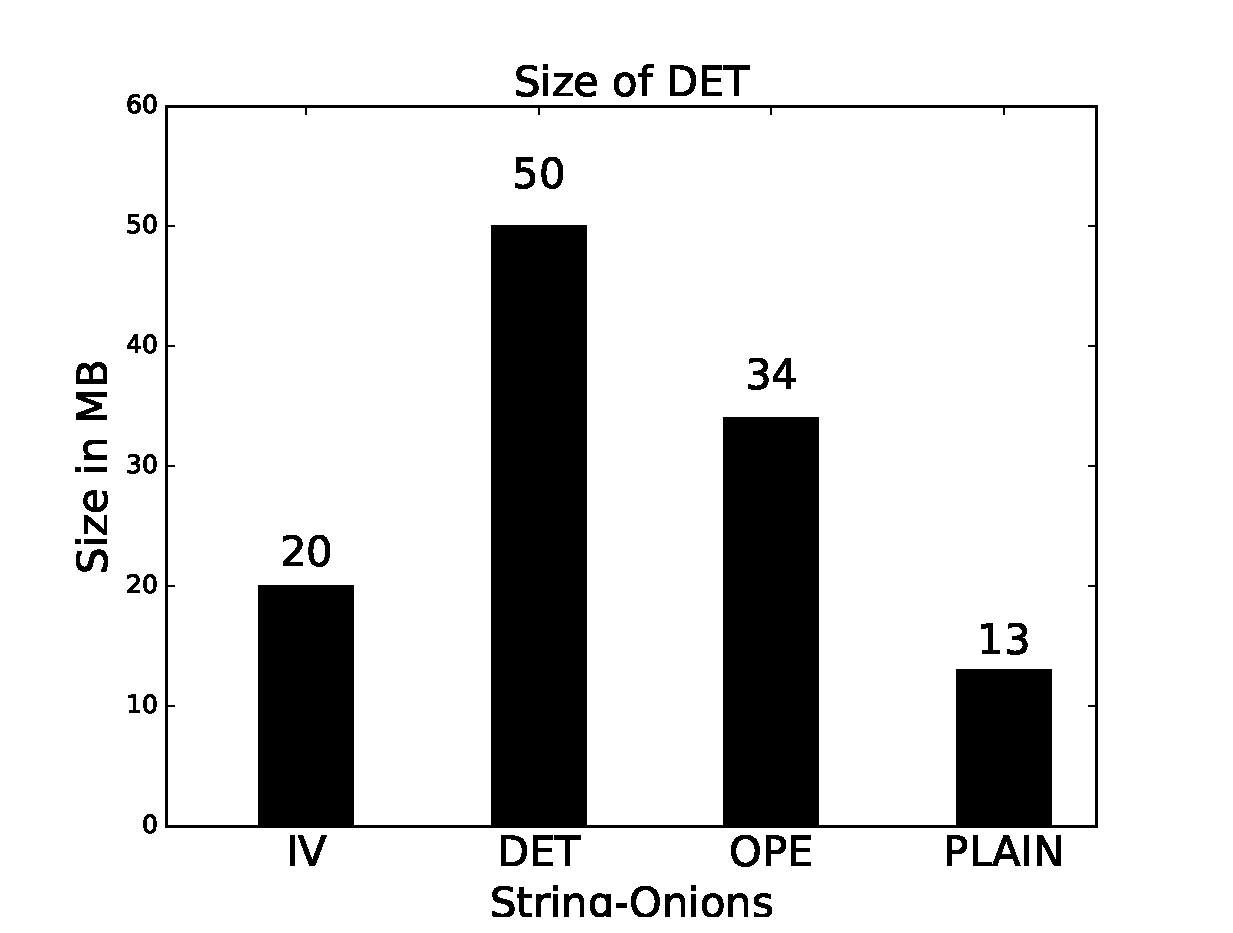
\includegraphics[width=4.7cm]{images/det-rnd.eps}   
    \caption{\small{This figure shows the size of each encrypted column in the form of text file for the table we creates that have one plaintext column of String type}} 
    \label{fig:stack12}   

  \end{minipage} 
\end{figure*}

% \begin{figure}[tb]
% \centering
% 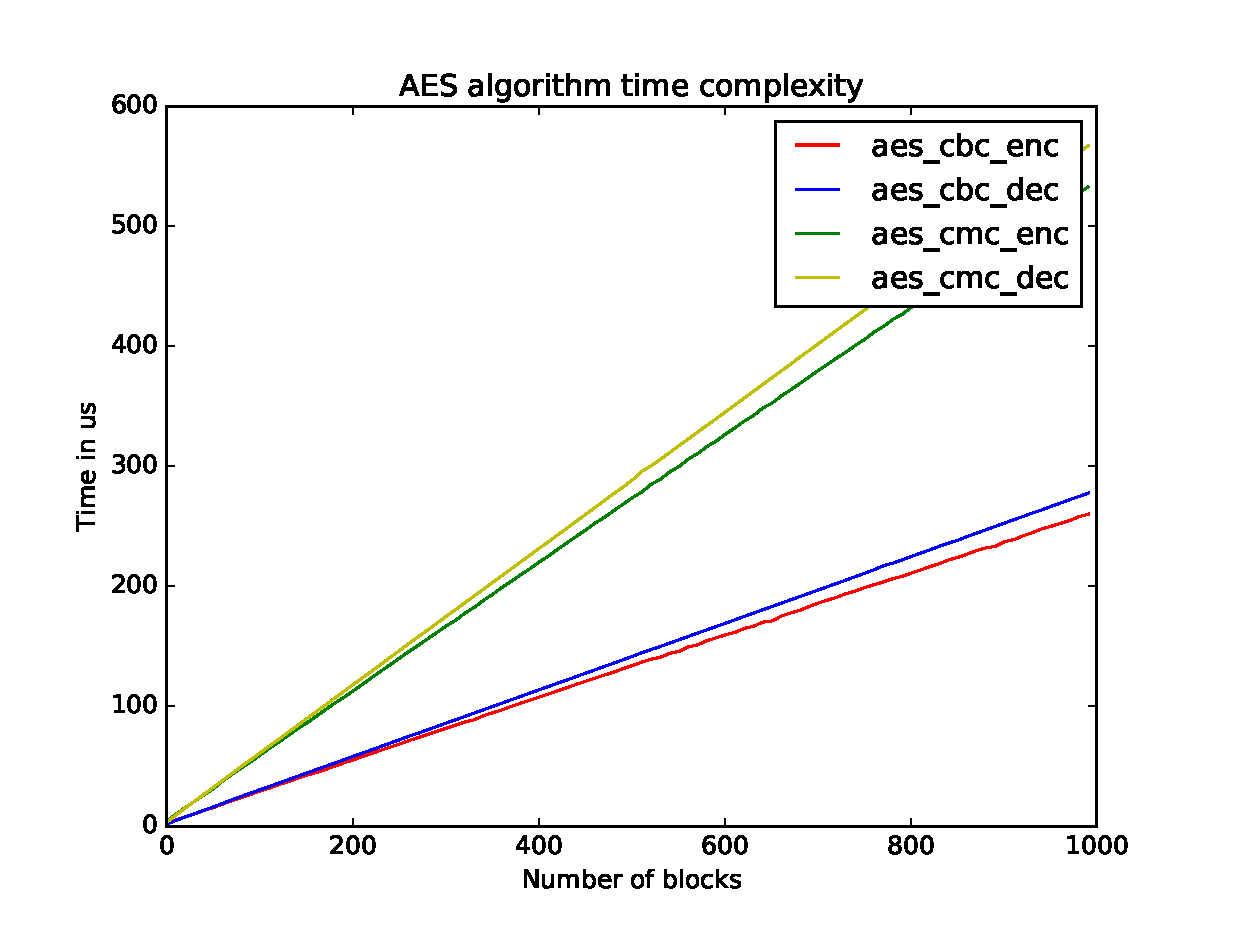
\includegraphics[width=8cm]{images/aes.eps}
% \caption{Aes time consumpation}
% \label{fig:stack9}
% \end{figure}




% \begin{figure}[tb]
% \centering
% 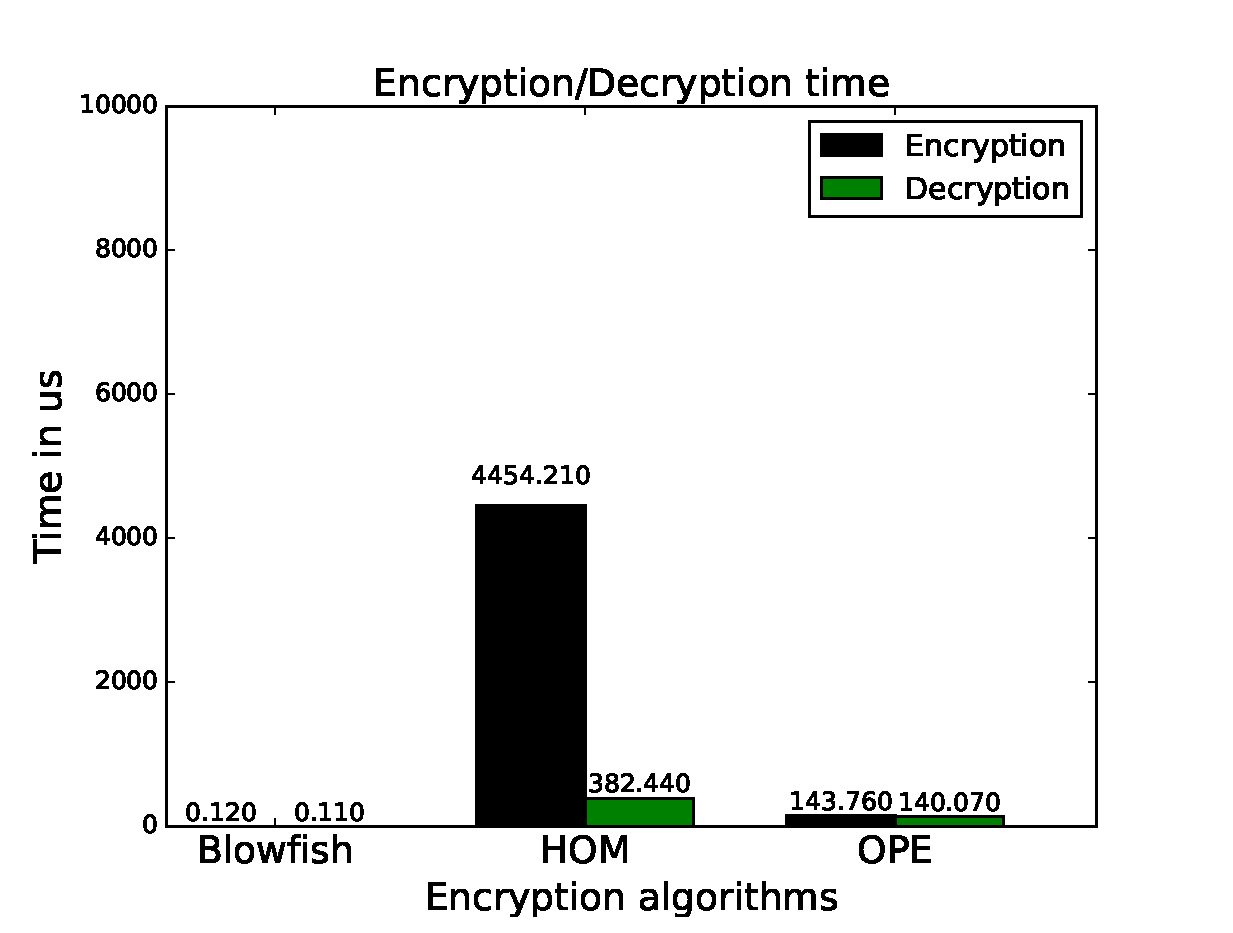
\includegraphics[width=8cm]{images/time.eps}
% \caption{time consumpation}
% \label{fig:stack10}
% \end{figure}


Figure~\ref{fig:stack9} shows the time consumption for encryption and decryption for AES-CBC and AES-CMC. AES-CBC is a simple wrapper of AES function in the open-ssl library, and AES-CMC is a wrapper of AES-CBC  which internally calls AES-CBC twice. So the time for encryption and decryption of AES-CMC is roughly twice that of AES-CBC, and the time consumption is almost proportional to the size of plaintext. Figure~\ref{fig:stack10} shows the encryption and decryption time for pailliar, blowfish, and the order preserving encryption. We can find that blowfish, which operate on 64 bits integer, is fast. OPE is also fast. HOM, which uses pailliar, is slow. 9.1ms is used for encryption, which means the throughput of inserting one column of integer is limited to around 100 rows per second.

We now begin to analyze the two type of data that is supported by CryptdDB. We create one simple table with only one field, and backup that encrypted data, and show the size of each encrypted onion. Note that this is not exactly the same as logical backup since in logical back, data is in the form of sql queries. We do not backup the data in SQL query form because the logically deduplicated queries, which are not complete, can not execute on the DBMS directly. So we choose to backup each column separately, something like the 'SELECT into file' method.

For integer data, as we mentioned before, the columns are replicated three time for three onions with an additional salt column for the decrypting the layer RND. We insert 1,000,000 integers, all of them are simple 12345. Figure~\ref{fig:stack11} shows the size of each onion when backed up. We dump each column into separate files and use 'du -h' to find the size of each column when in string representation. We can find that HOM is the biggest, since it's data type: varbinary(256), when in string representation, occupies large space. IV is random 64 bits integer, DET is also random 64 bits integer, so they are of similar size. OPE is larger than DET, since the type is varbinary(32) in rnd layer. 


% \begin{figure}[tb]
% \centering
% 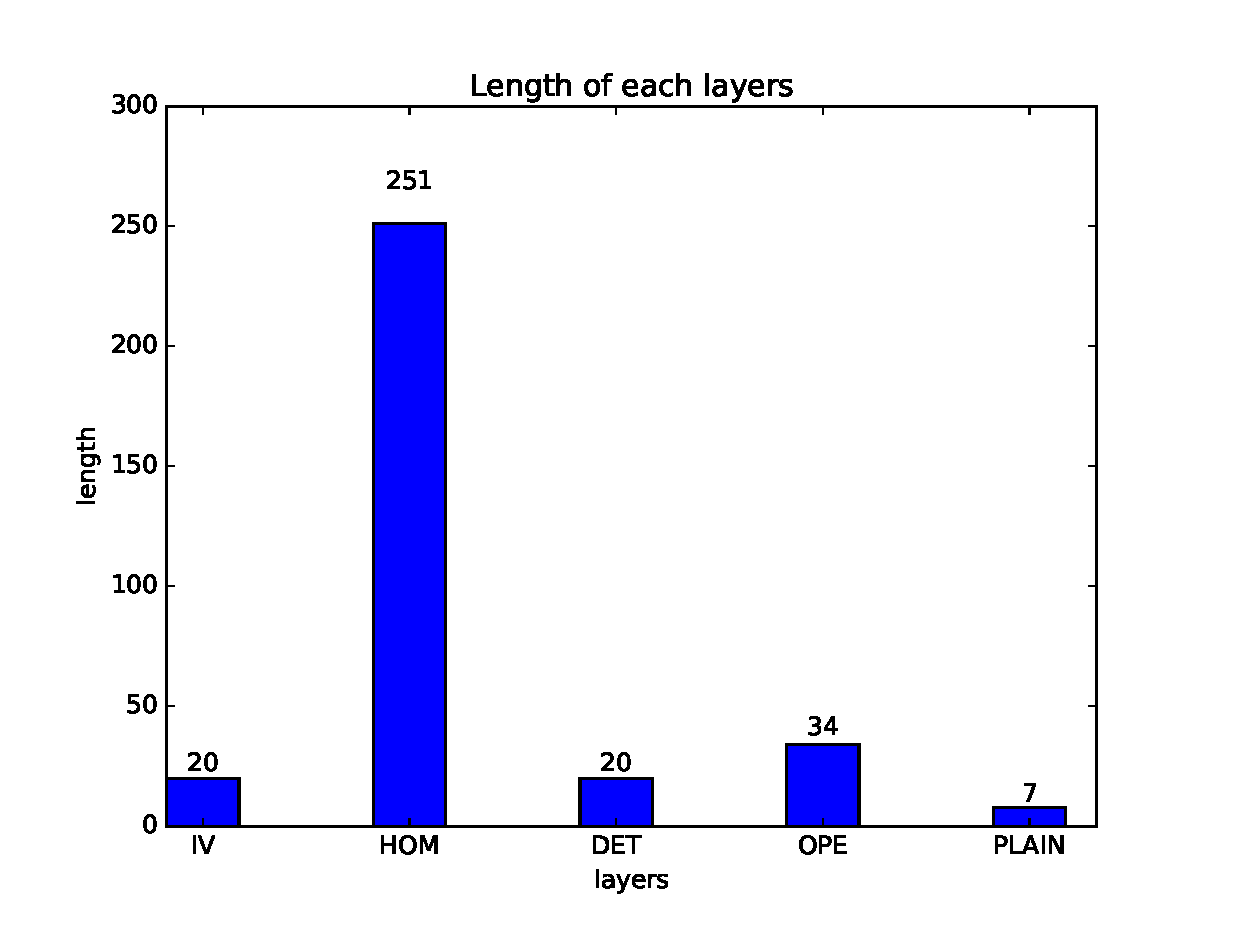
\includegraphics[width=8cm]{images/size-of-each-onion.eps}
% \caption{Size of onion for integer type}
% \label{fig:stack11}
% \end{figure}



\begin{figure}   
  \begin{minipage}[t]{0.47\columnwidth}  
    \centering   

    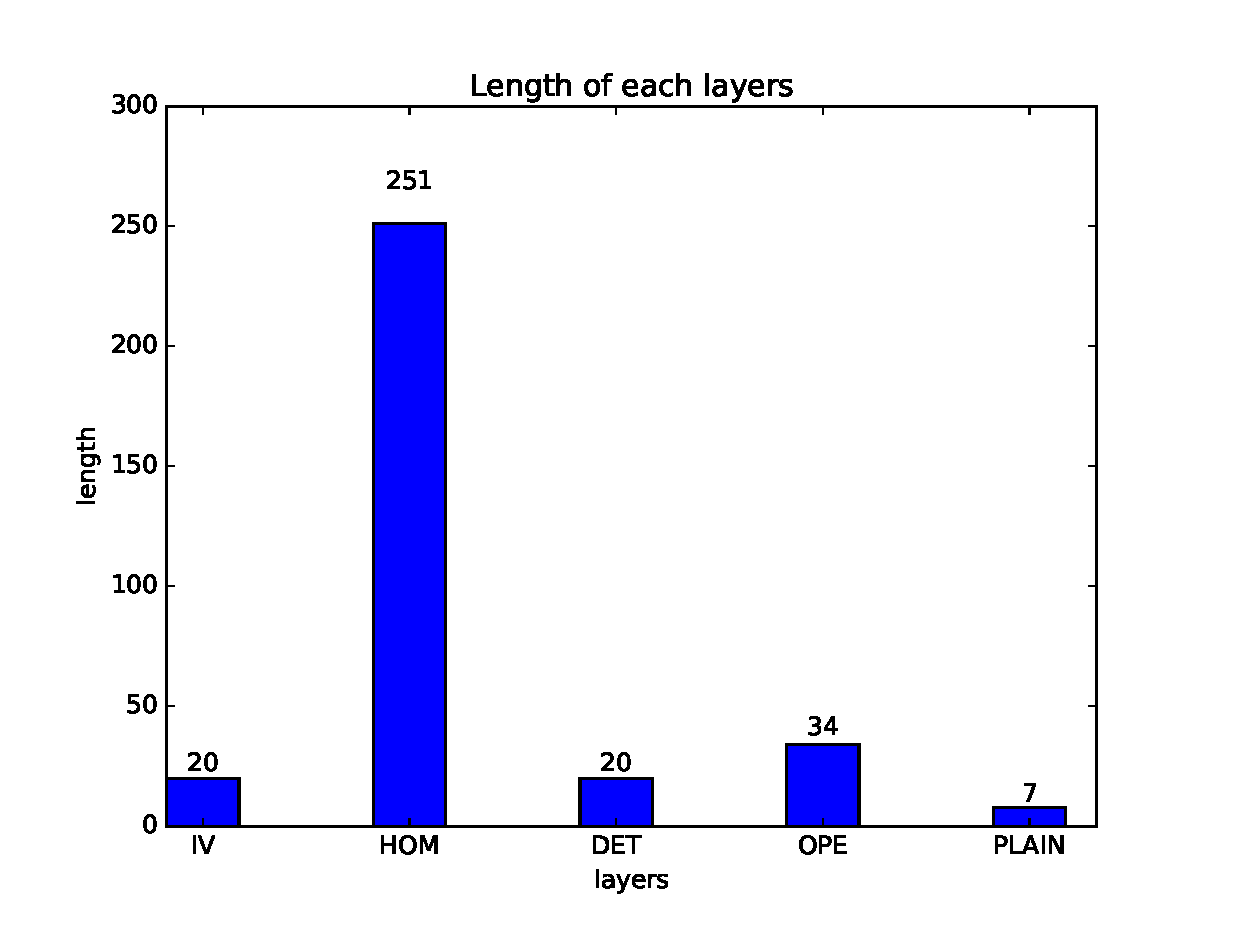
\includegraphics[width=4.7cm]{images/size-of-each-onion.eps}   
    \caption{\small{This figure shows the size of each encrypted column in the form of text file for the table we creates that has one plaintext column of Integer type}} 
    \label{fig:stack11}   
  \end{minipage}%  
  \hfill 
  \begin{minipage}[t]{0.47\columnwidth}   
    \centering   
    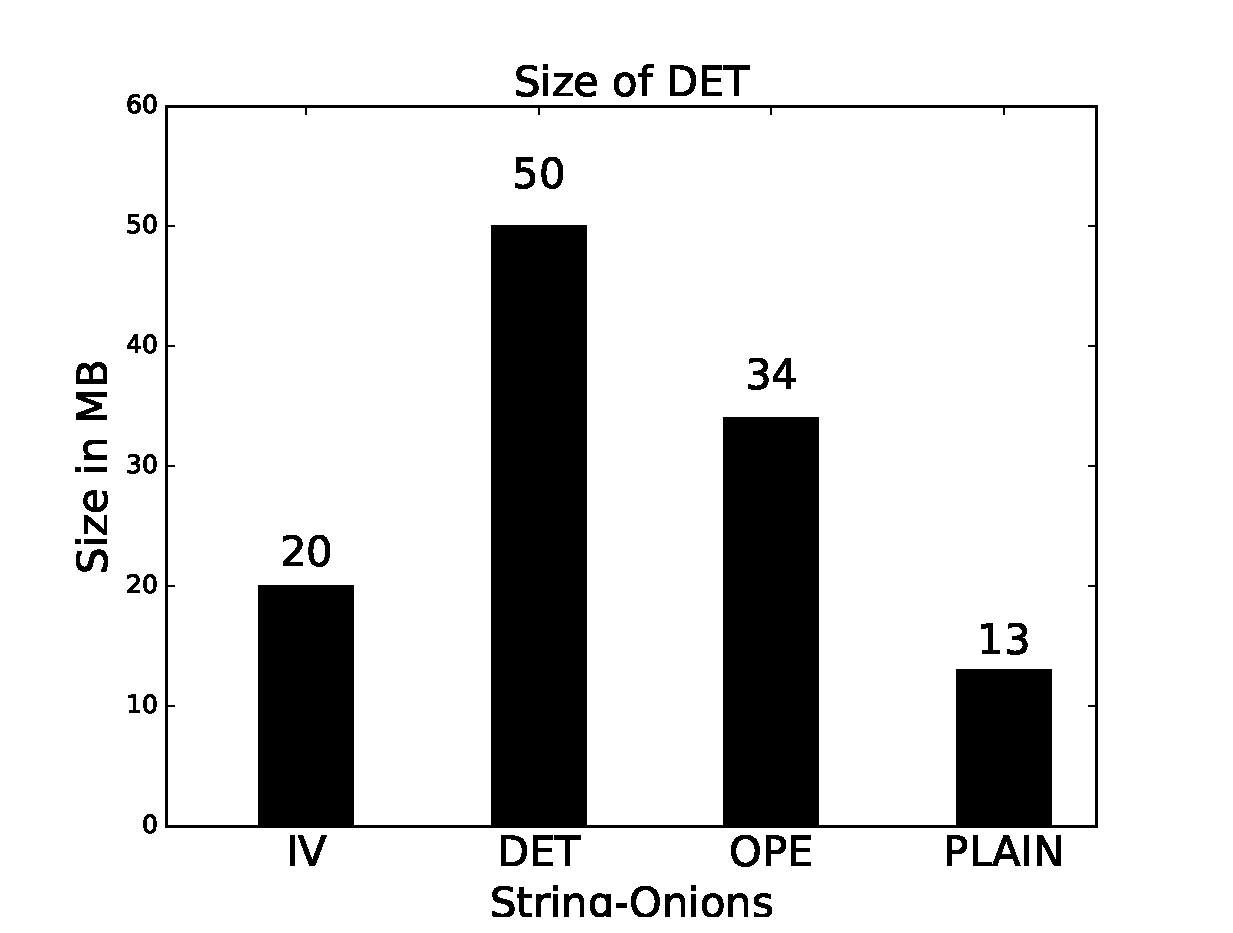
\includegraphics[width=4.7cm]{images/det-rnd.eps}   
    \caption{\small{This figure shows the size of each encrypted column in the form of text file for the table we creates that have one plaintext column of String type}} 
    \label{fig:stack12}   

  \end{minipage}   
\end{figure}





For string type, we do experiment with a simple table of varchar(10). After encryption, the onion DET will be tranformed to varbinary(48) due to the padding, and OPE will be varbinary(32), salt should be big int. We insert 1,000,000 plaintext of length 10 into the table, and the figure~\ref{fig:stack12} depicts the results for each column.We can find that even for very short string, three layer of encryption in onion DET can make it larger than the onion OPE. So ope is always assumed  smaller than DET. And the size of salt remains the same as in the experiment with integers. We can find that decrypting the RND layer can produce greater compression ratio. We use gizp with default options. This is an extream case since all the data in the columns are the same. For a big column with low Cardinality, like gender, this approach is expected to produce similar results. 


% \begin{figure}[tb]
% \centering
% 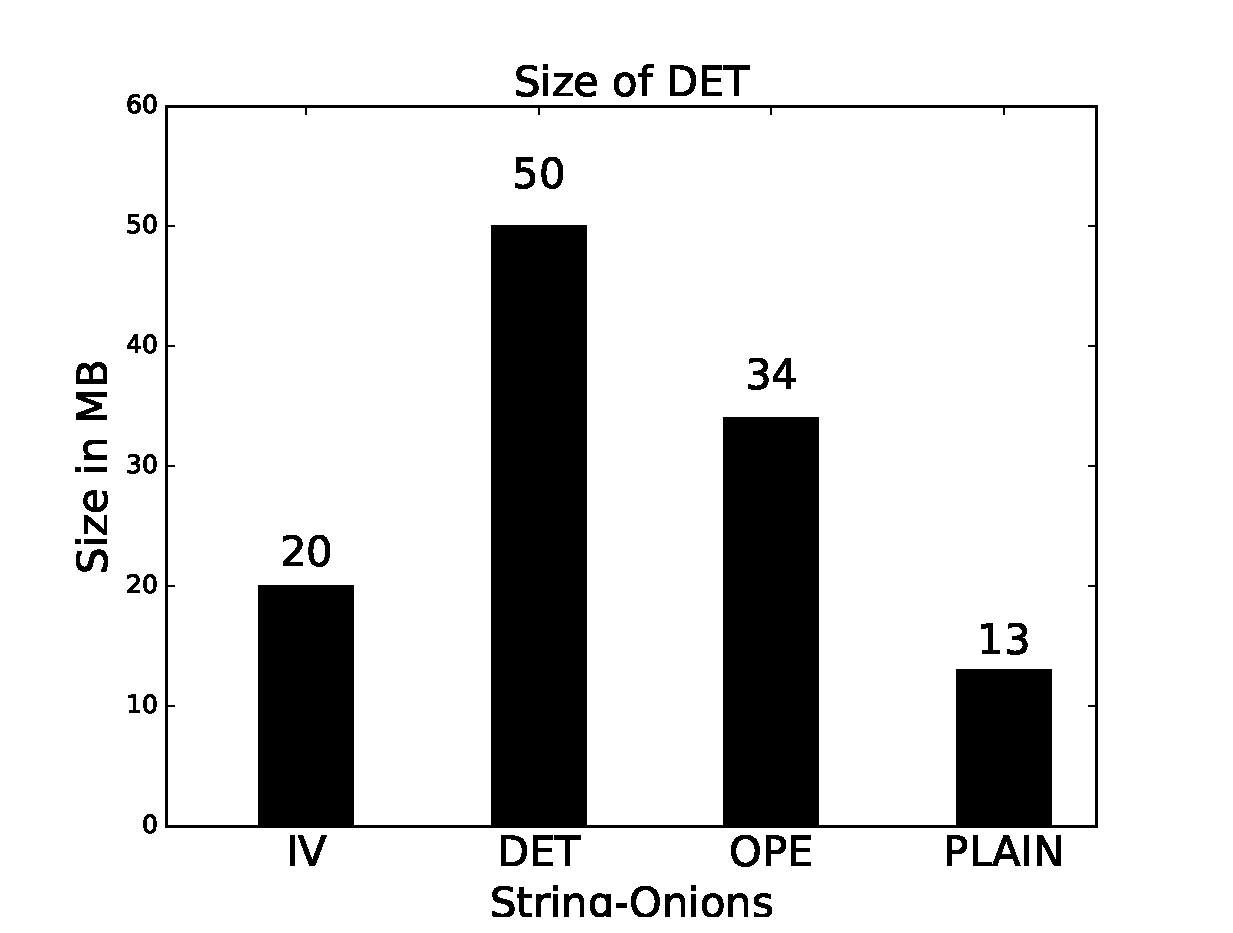
\includegraphics[width=8cm]{images/det-rnd.eps}
% \caption{size of onion for string type}
% \label{fig:stack12}
% \end{figure}







% \begin{figure}[tb]
% \centering
% 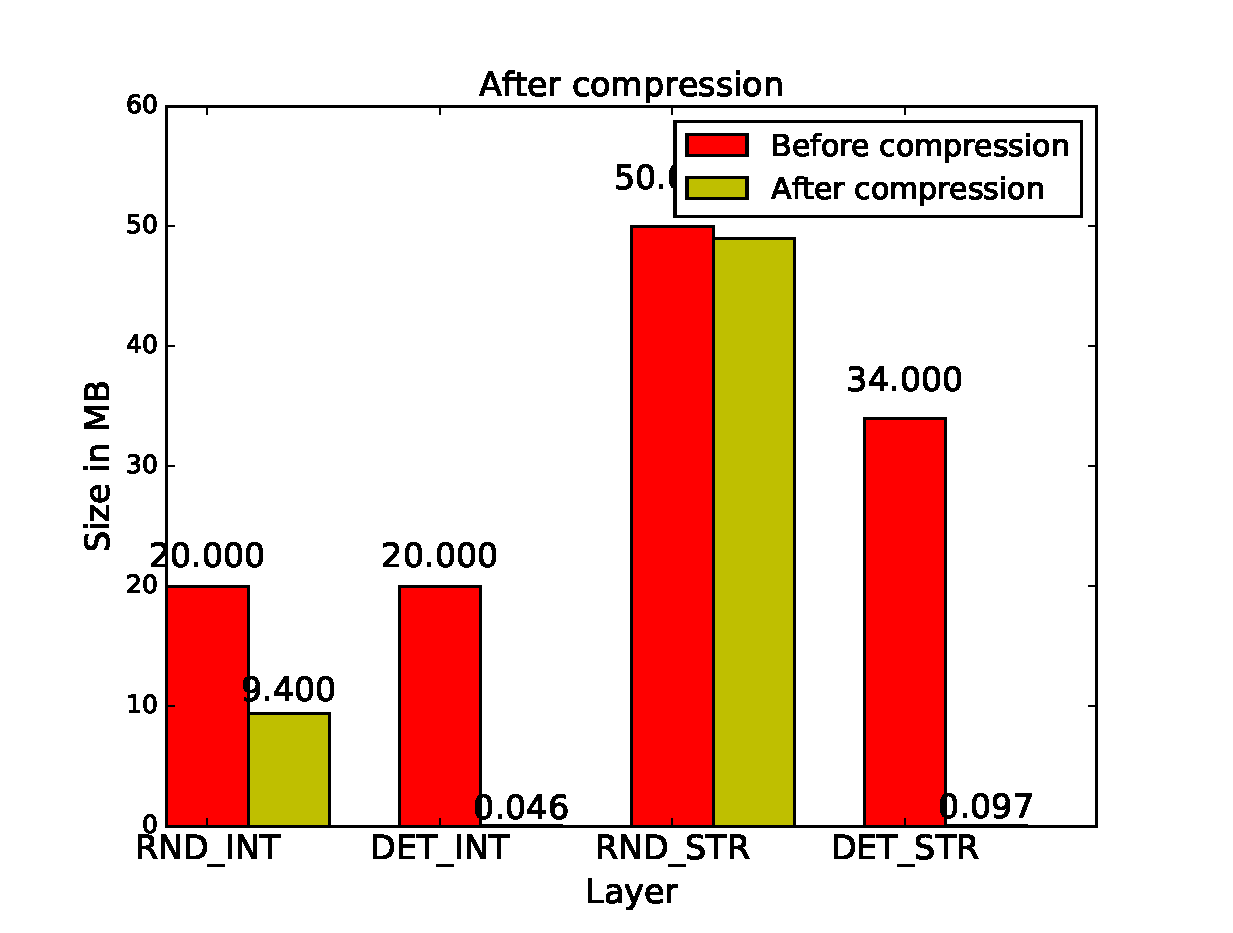
\includegraphics[width=8cm]{images/aftercompression.eps}
% \caption{size of onion for string type}
% \label{fig:stack12}
% \end{figure}


We also give the expected recovery time for each onion based on the assumpation that we only backup the Onion DET. Figure~\ref{fig:stack12} depicts the results.


Finally we do experiment with the TPCC-MySQL, the original data is the 74MB, and the encrypted data is 1.5 GB. So there is large expansion. especially for those tables that has columns of integers of small value like 0,1. Those could be stored with 1 Bytes should now pay the 256 Bytes overhead of the onion HOM, inaddition to other onions and the IV column. We can use the simplest method to backup only the DET and IV column, which is 229M(DET)+125M(IV). 
% Figure~\ref{fig:stack13} depicts the results. As we have mentioned, analyzing a table can be easy since the characteristics of each column is known. 


% \begin{figure}[tb]
% \centering
% 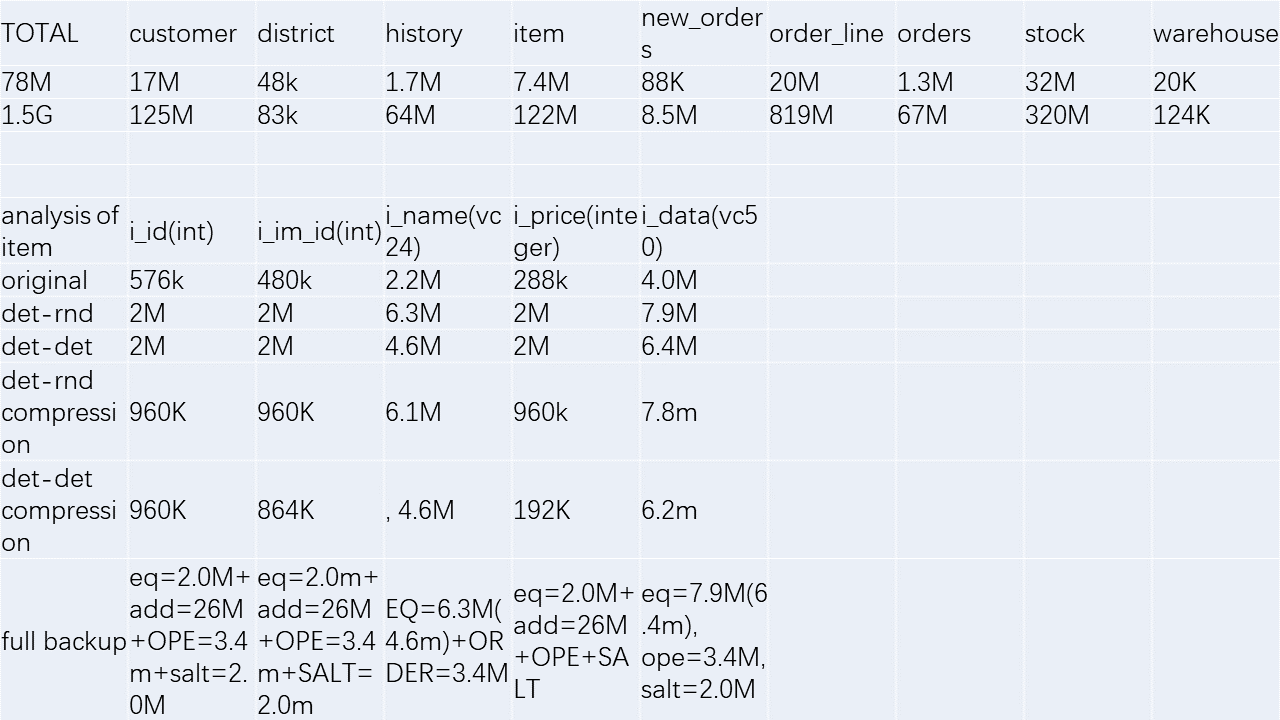
\includegraphics[width=8cm]{images/tpcc.png}
% \caption{tpcc data}
% \label{fig:stack13}
% \end{figure}





Based on the above results, we can find that, in the current implementation of CryptDB, Onion OPE is always small and can not be used for recovering, So OPE can be removed  to save space. For integers, the onion HOM is large, and also taken a long time to recover, So If we remove HOM for deduplication, and use the onion DET for recovering the data, we can save a lot space while paying the overhead of recomputing the onion HOM. If we can find ways to accelerate the computation of pailliar, then this deduplication can be more efficient. The onion DET-INT uses blowfish, which is fast and occupy little space compared to the plaintext, so it's reasonable to retain this onion. Decrypting the layer RND-int should reduce the size by half since we no longer need the IV column, so we can remove this column. Also, decrypting the RND-int layers can produce higher compression ratio. Things are similar for string type. String type has a search onion, which is expected to be similar to onion DET. So if we remove search, we expect to reduce the size by half. If we then remove the RND-STR layer, we also get higher compression ratio. In \citep{popa2015guidelines}, new onions are added in CryptDB, this can leave more space for deduplication.

\begin{figure}   
  \begin{minipage}[t]{0.5\linewidth}  
    \centering   
    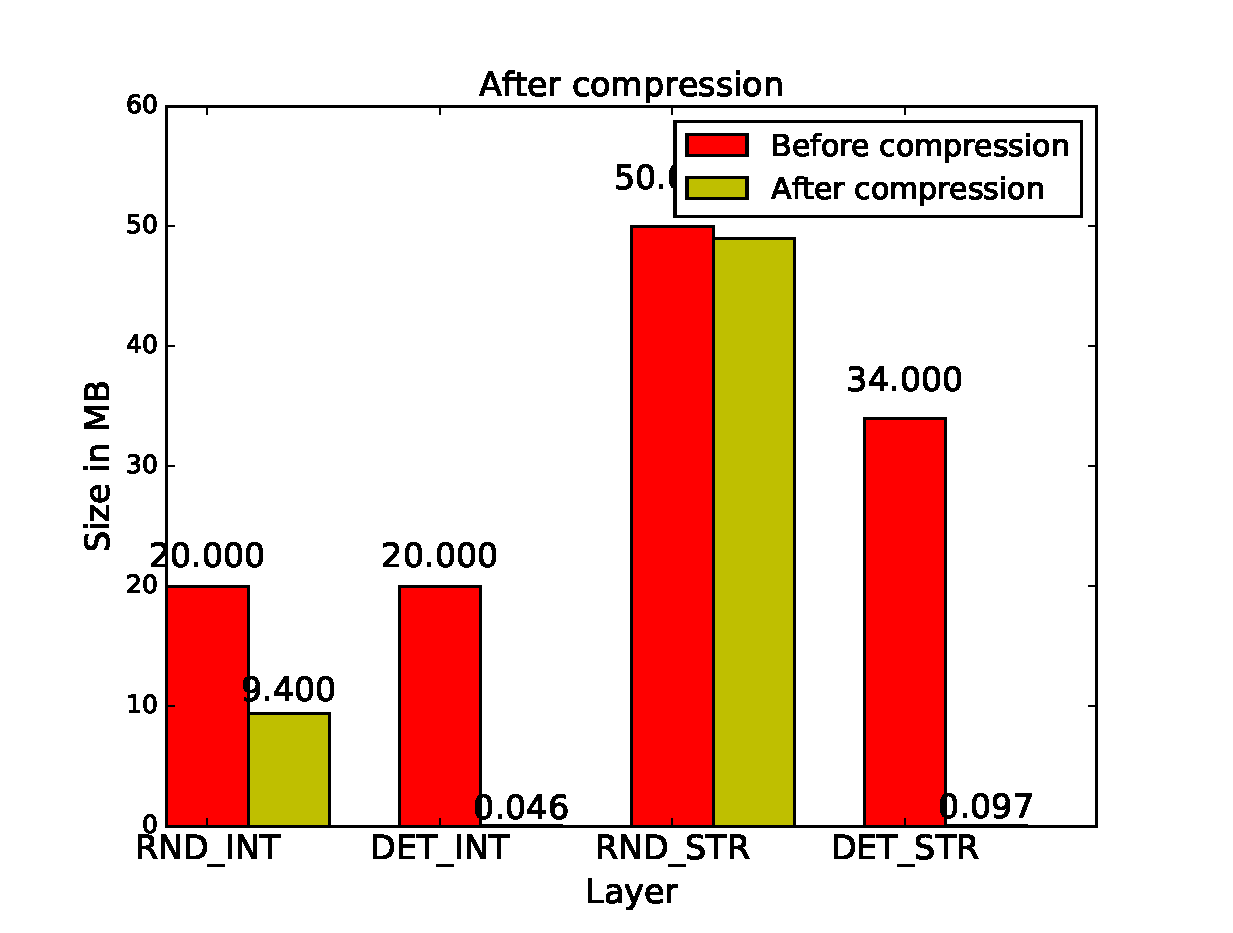
\includegraphics[width=4.7cm]{images/aftercompression.eps}   
    \caption{\small{This figure shows how the size of each encrypted column change after being compressed using gzip}} 
    \label{fig:stack12}   
  \end{minipage}%   
  % \begin{minipage}[t]{0.5\linewidth}   
  %   \centering   
  %   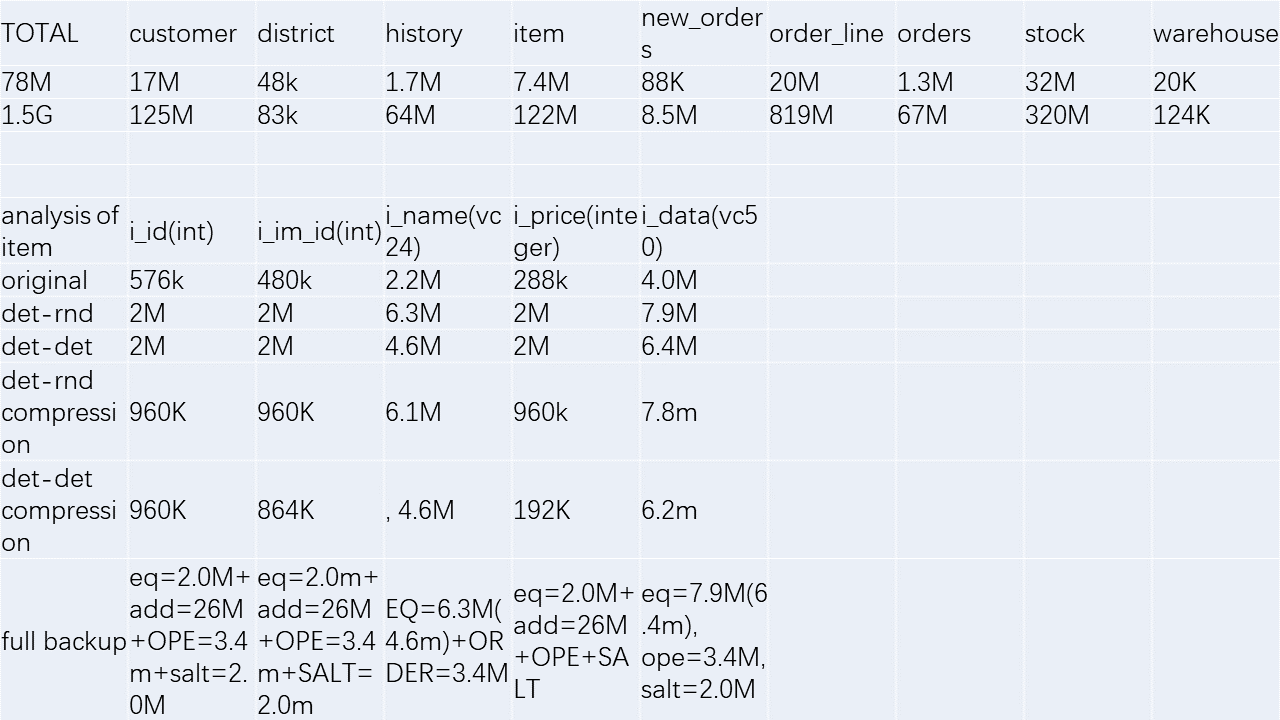
\includegraphics[width=4.0cm]{images/tpcc.png}   
  %   \caption{tpcc}   
  %   \label{fig:side:b}   
  % \end{minipage}   
\end{figure}
% \begin{talbe*}
% \begin{tabu*} to \hsize {|X|X|X|X|X|X|X|X|X|X|}
% \hline
% Tablename & customer & district & history& item & new\_order & order\_line& orders & stock & warehouse \\ \hline
% DET & 1 & 2 & 3& 1 & 2 & 3& 1 & 2 & 3 \\ \hline
% OPE & 1 & 2 & 3& 1 & 2 & 3& 1 & 2 & 3\\ \hline
% HOM & 1 & 2 & 3& 1 & 2 & 3& 1 & 2 & 3 \\ \hline
% IV & 1 & 2 & 3 & 1 & 2 & 3& 1 & 2 & 3\\ \hline
% TOTAL & 1 & 2 & 3 & 1 & 2 & 3& 1 & 2 & 3\\ \hline
% \end{tabu*}
% \end{table*}

% % \begin{talbe*}
% \begin{tabular}{ccc}
% \toprule
% 2&9&4\\
% \midrule
% 7&5&3\\
% 6&1&8\\
% \bottomrule
% \end{tabular}
% % \end{table*}



% \begin{table*}
% \renewcommand{\arraystretch}{1.3}
% \label{tab:example}
% \centering
% \begin{tabular}{|c|c|c|c|c|c|c|c|c|c|c|}
%   \hline
%   % after \\: \hline or \cline{col1-col2} \cline{col3-col4} ...
% &total & customer & district & history & item & new\_order & order\_line & orders & stock & warehouse   \\
% DET &  & 13M+9M+5.1M+3.8M+9*608K & 1 & 1 & 1 & 1 & 1 & 1 & 1&1 \\  
% OPE &  & 13*976k+8*608k & 1 & 1 & 1 & 1 & 1 & 1 & 1&1 \\
% HOM &  & 7.4M*9 & 1 & 1 & 1 & 1 & 1 & 1 & 1&1 \\
% IV &  & 608k*21 & 1 & 1 & 1 & 1 & 1 & 1 & 1&1 \\
% \hline
% \end{tabular}
% \caption{This table shows the size of each of tcpp-mysql's table's onions and IV column}
% \end{table*}